\section{Prospective engineering improvements}
After the failed memory gate, we initiated separately authorized improvement studies. Each new protocol was committed before its development run, used new development and confirmation seeds, and preserved preceding failures. These are an adaptive sequence of engineering studies, not repetitions of an unchanged sealed test. Interval adjustments apply within each study, not across the entire research sequence.

All new runs retain rule steering, seven-tic decisions, the 180-window cap and the 0.25 cost per issued-fire window. The primary net utility subtracts one unit per second of decision compute, excluding engine observation/advance and trace I/O. Lightweight coding and reporting ran concurrently on the workstation; timing remains a screening measurement. The confirmation rule requires at least 0.5 mean net-utility gain and a positive lower interval endpoint against rules and the five historical history-MAP fits in both scenarios. It additionally requires each kill-difference lower endpoint to exceed $-1$, and every selected-controller episode's p95 decision time to remain below 1 ms. Eight primary contrasts use 20,000 paired bootstrap draws and 99.375\% percentile intervals; history comparisons resample both seeds and training fits. These finite-sample intervals are exploratory.

\subsection{Ammo-only cadence}
The first new study, frozen at \texttt{5bd0a64}, screened nine fixed aiming/cadence variants on 24 new Center seeds. Eligible candidates needed at least 0.5 mean net-utility gain and no more than 0.5 mean kill loss against rules. Only a one-window rest following observed ammo consumption qualified. It gained 0.750 utility while preserving mean kills at 6.5. Tighter-aim alternatives with higher utility failed the kill requirement.

Confirmation used 96 new seeds per scenario, the selected rule, original rules, a matched no-rest control, a command-rest control and five historical history fits, totaling 1,728 episodes. The selected policy gained 0.854 net utility over rules in Center (interval $[0.672,1.050]$), with identical paired kills. It had identical gameplay outcomes to rules in Line: ammo replenishment hides expenditure in that scenario. Against the history-model bank, utility and kill criteria were not all established. The full gate failed. The confirmation does establish a narrow gain over rules in Center, without implying improved kills or per-shot accuracy.

\subsection{Complementary observable events}
A separate fixed candidate, frozen at \texttt{337629c}, combines an observed ammo decrease with the preceding window's hit feedback. Either event triggers the same one-window rest. Ammo can identify a missed shot; hit feedback remains observable when replenishment masks expenditure. This controller reads no hidden weapon readiness and no future outcome.

The five development arms were combined events, rules, ammo only, hit only and command rest, each evaluated on 24 new seeds in both scenarios. The fixed combination qualified: utility gains were 0.792 in Center and 5.823 in Line, with identical kills. Confirmation then evaluated those five policies and five historical history fits on 96 fresh seeds per scenario, totaling 1,920 episodes.

The combination gained 0.823 net utility over rules in Center ($[0.643,1.025]$), and 5.435 in Line ($[4.812,6.070]$). Kills matched rules in all 192 paired episodes. Ammo-only matched the combination in Center and hit-only matched it in Line. However, comparisons against the history-model bank still failed the full gate: utility intervals included zero in both scenarios, and kill noninferiority was not established. A command-rest control remained stronger on Line. These results support an event-memory engineering baseline, not superiority over every control.

\begin{figure}[H]
\centering
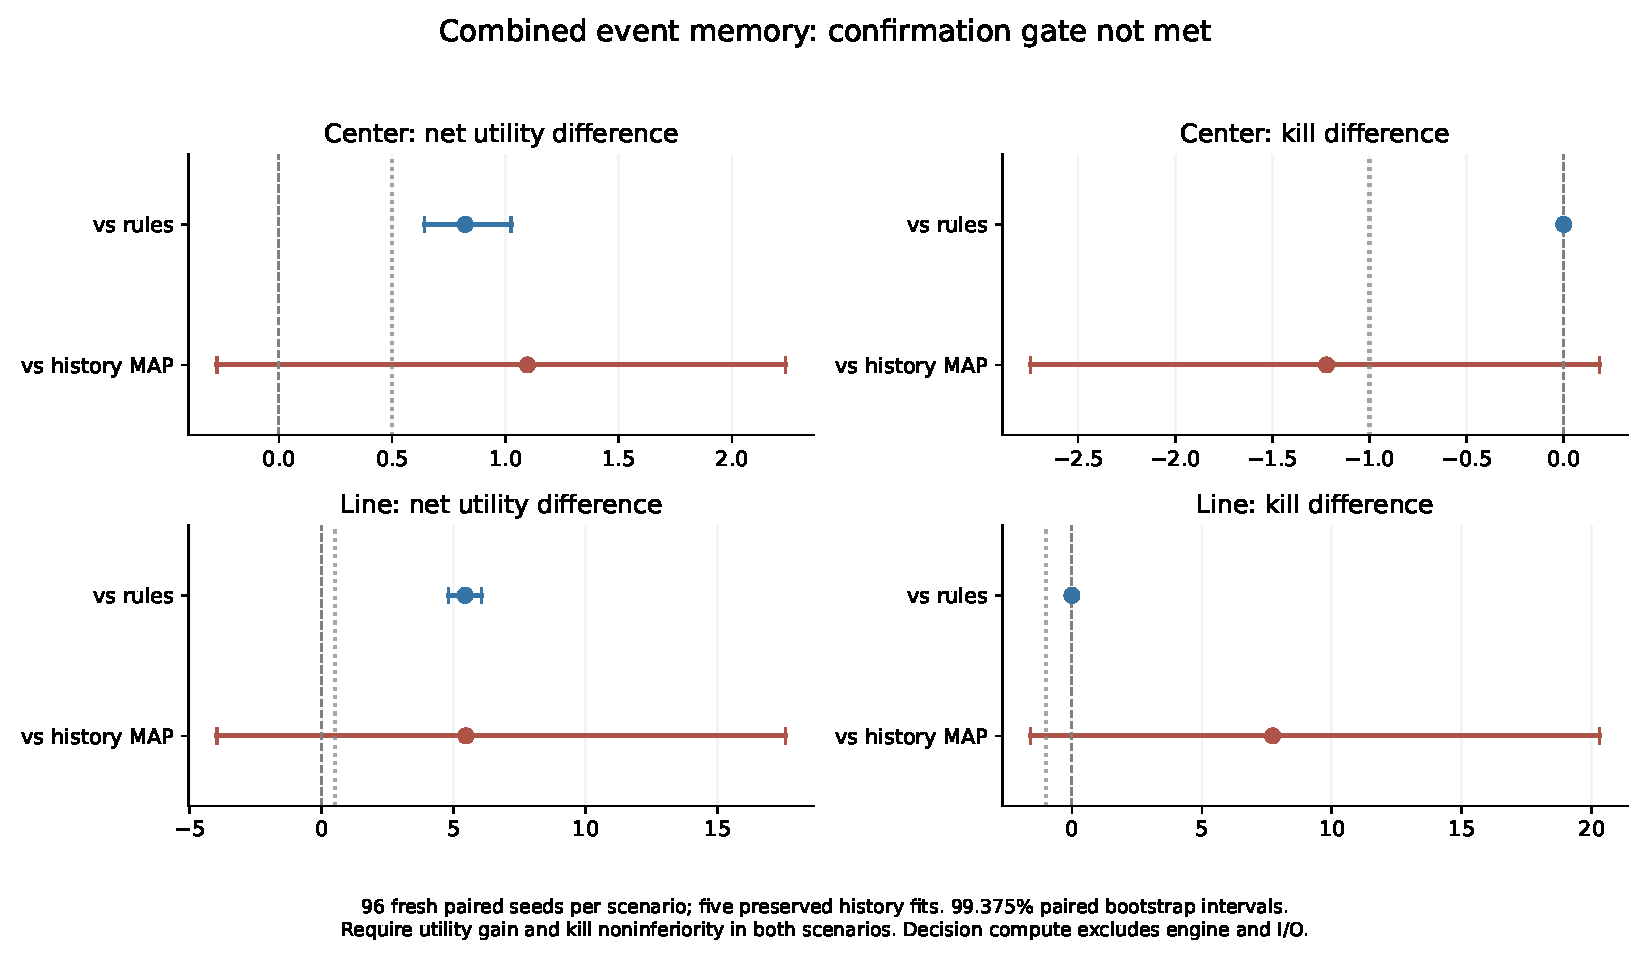
\includegraphics[width=\linewidth]{../evidence/event-cadence-doom-v1/confirmation-contrasts.pdf}
\caption{Combined observable-event memory: confirmed command-utility gains over rules, with unchanged paired kills, but a failed broader gate against the history-model bank. Dashed lines mark zero; dotted lines mark the 0.5 mean utility threshold or the $-1$ kill noninferiority boundary.}
\end{figure}

\subsection{Matched ensembles and portable representations}
The third study was frozen at \texttt{6402a29}. Historical training was Center-only, and individual models transferred inconsistently to Line. The new current representation uses four features: bias, visibility, capped aim error divided by a target-width tolerance, and target width. It removes absolute ammo, health and distance. A history variant adds previous fire, previous hit, capped age since fire and a history-present bit, giving eight features. This changes both inputs and representation geometry, so it does not isolate a single variable as the mechanism.

All fitted ensembles reuse exactly the same 80 historical episodes, five training splits, issued-fire labels, Gaussian prior and optimizer. Each ensemble averages five MAP probabilities. Controls include an ensemble of the original 17-feature models, ruling out model averaging as an automatic explanation for representation-specific claims. All ensemble controls require a visible target; the unchanged historical single-model references retain their original behavior.

Eight arms with and without event memory were evaluated on 24 new seeds per scenario. Selection maximized the smaller of the two scenario gains among candidates passing the development utility and kill screens. The four-feature current-state ensemble with explicit event memory qualified, with development gains of 3.520 utility and 2.708 kills in Center, and 7.352 utility and 1.167 kills in Line. Learned-history variants were weaker on this criterion. These development results selected one candidate for confirmation.

Fresh confirmation ran 1,920 episodes, using 96 new seeds per scenario and ten arms counting the historical fits separately. Against rules, net-utility gains were 2.322 in Center ($[1.549,3.129]$) and 5.663 in Line ($[3.590,7.858]$). The full gate nevertheless failed. Center kill noninferiority against the historical bank was unresolved: difference 0.083, interval $[-1.440,1.734]$. On Line, kill noninferiority against rules was also unresolved: $-0.635$, interval $[-2.146,0.875]$. The Line utility interval against the historical bank included zero. Both latency screens passed.

Secondary comparisons isolate the explicit event gate. Against the same fitted head without this gate, net-utility gains were 0.760 in Center ($[0.575,0.961]$) and 4.846 in Line ($[4.236,5.466]$), with kills identical in every one of the 192 paired episodes. These secondary intervals are exploratory and outside the eight-primary-comparison correction family. The gate avoids redundant issued-fire windows while preserving successful windows; this is reduced command cost, not established ammunition savings or improved combat performance. Against the original matched ensemble, the selected policy gained 3.271 utility in Center ($[2.386,4.134]$), but averaged $-2.228$ on Line ($[-4.437,0.015]$). The representation does not dominate across scenarios.

\begin{figure}[H]
\centering
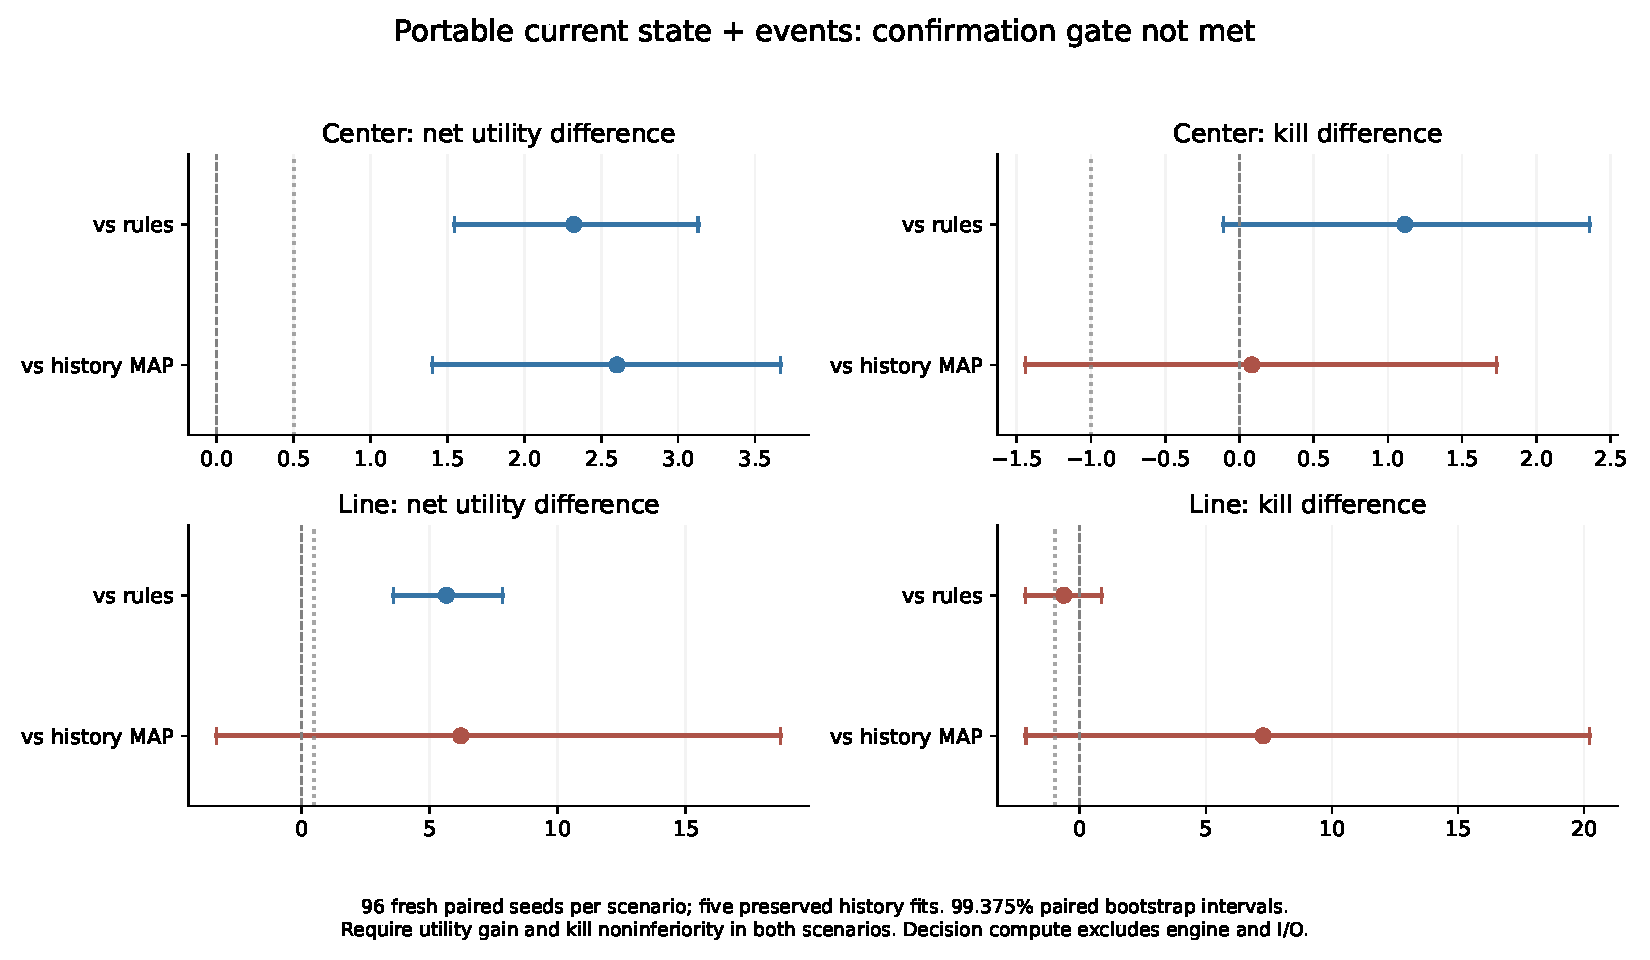
\includegraphics[width=\linewidth]{../evidence/portable-head-doom-v1/confirmation-contrasts.pdf}
\caption{Fresh confirmation of the selected portable current-state ensemble with event memory. Utility gains over rules coexist with unresolved kill noninferiority and historical-bank comparisons. The full gate failed.}
\end{figure}

Taken together, the three prospective studies add 6,408 episodes and support a modest engineering baseline. None passes the broader continuation rule. Both scenarios were used in the last two development stages, so their confirmation is fresh-seed testing, not unseen-task validation. Reducing a costly but ineffectual fire command is useful under this utility definition; it does not by itself establish a general memory mechanism.

The relevant precedent includes learned action repetition and temporal abstraction \citep{lakshminarayanan2017dynamic,sharma2017figar}. Our cadence studies keep decision windows fixed and use simple observed feedback; they are not reproductions of those methods or a novel temporal abstraction algorithm. These studies establish no new Bayesian, recurrent, or language-model RL method and no ICLR novelty.
